
\section{Operadores Genéricos}

% >8----------------------------EXEMPLO DO QUE QUEREMOS FAZER----------------------------8<
\begin{frame}
  \begin{center}
    \textit{It seems to me that one of the biggest problems people have with programs is writing programs that are dead ends. What I mean by dead end is: you've written this big complicated piece of software and then the world changes [...] and then you have to rewrite out a big chunk of it.}\\
        --- Gerald Jay Sussman.
    \end{center}
\end{frame}

\begin{frame}[fragile]
  \frametitle{Exemplo de Uso dos Pares}

  \begin{itemize}
    \item Sistema aritmético flexível e extensível.
  \end{itemize}

  \pause

  \[\dfrac{(2.3 + 1i) + \left(\dfrac{2}{3} \times 5.2\right)}{(2.8 + 0.5i)}\]
  \vspace{2em}
  \pause

  \begin{code}
              (div (add (C ((R 2.3) (R 1)))
                        (mul (Q ((Z 2) (Z 3)))
                             (R 5.2)))
                   (C ((R 2.8) (R 0.5))))
  \end{code}
  \vspace{1em}
\end{frame}
% >8----------------------------EXEMPLO DO QUE QUEREMOS FAZER----------------------------8<


% >8---------------------------------O QUE QUEREMOS FAZER--------------------------------8<
\begin{frame}
  \frametitle{Sistema Aritmético}
    \begin{itemize}
      \item Operadores: $+, -, *, /$ \\
      \vspace{0.5em}
      \begin{itemize}
        \item $+ \,\,:\,\, \mapsto \,\,$\texttt{add}
        \item $- \,\,:\,\, \mapsto \,\,$\texttt{sub}
        \item $* \,\,:\,\, \mapsto \,\,$\texttt{mul}
        \item $/ \,\,:\,\, \mapsto \,\,$\texttt{div}
      \end{itemize}
      \pause

      \vspace{1.3em}
      \item Operandos: $\mathbb{Z}, \mathbb{Q}, \mathbb{R}\text{ e }\mathbb{C}$
      \vspace{0.5em}
      \begin{itemize}
        \item $\mathbb{Z}\,\,:\,\,(x)\,\,\mapsto\,\,$ \texttt{(Z x)} \\
        \vspace{0.5em}
        \item $\mathbb{Q}\,\,:\,\,(\frac{x}{y})\,\,\mapsto\,\,$ \texttt{(Q ((Z x) (Z y)))} \\
        \vspace{0.5em}
        \item $\mathbb{R}\,\,:\,\,(x) \,\,\mapsto\,\,$ \texttt{(R x)} \\
        \vspace{0.5em}
        \item $\mathbb{C}\,\,:\,\,(x + yi) \,\,\mapsto\,\,$ \texttt{(C ((R x) (R y)))} \\
      \end{itemize}
    \end{itemize}
\end{frame}
% >8--------------------------------O QUE QUEREMOS FAZER---------------------------------8<



% >8--------------------------PROCEDIMENTO DE ADIÇÃO DE INTEIROS-------------------------8<
\begin{frame}[fragile]
  \frametitle{Operadores Aritméticos}
  \framesubtitle{Exemplo: Adição de Inteiros}
  \begin{minipage}{0.47\textwidth}
  \begin{code}
(define (add-int x y)
  (cons Z (+ (cdr x)
             (cdr y))))
  \end{code}
  \end{minipage}
  \pause
  \hfill
  \begin{minipage}{0.47\textwidth}

  \vspace{0.5cm}
  \begin{code}
>> (add-int (Z 2) (Z 1))
  \end{code}
  \pause
  \vspace{0.07cm}
  \begin{code}
(cons Z (+ (cdr (Z 2))
           (cdr (Z 1))))
  \end{code}

  \pause
  \vspace{0.07cm}
  \begin{code}
(cons Z (+ 2 1))
  \end{code}

  \pause
  \vspace{0.07cm}
  \begin{code}
(cons Z 3)
  \end{code}

  \pause
  \vspace{0.07cm}
  \begin{code}
(Z 3)
  \end{code}
  \end{minipage}
\end{frame}
% >8--------------------------PROCEDIMENTO DE ADIÇÃO DE INTEIROS-------------------------8<



% >8----------------------------OUTROS PROCEDIMENTOS DE ADIÇÃO---------------------------8<
\begin{frame}[fragile]
  \frametitle{Operadores Aritméticos}
  \framesubtitle{Outros Procedimentos de Adição}
  \begin{minipage}{0.50\textwidth}
    \begin{code}
(define (add-rational x y)
  ...)
    \end{code}
    \pause

    \vspace{1.0cm}
    \begin{code}
(define (add-real x y)
  ...)
    \end{code}
    \pause

    \vspace{1.0cm}
    \begin{code}
(define (add-complex x y)
  ...)
    \end{code}
    \pause

  \end{minipage}
  \hfill
  \begin{minipage}{0.45\textwidth}
    Suas definições são triviais

    \pause

    \vspace{0.75cm}
    $\dfrac{a}{b}\,\,+\,\,\dfrac{x}{y}\,\,=\,\,\dfrac{ay + bx}{by}$

    \vspace{0.75cm}
    $a + b = (a + b)$

    \vspace{0.75cm}
    $(a + bi)\,+\,(x + yi) =$\\
    $(a + x)\,+\,(b + y)i$
  \end{minipage}
\end{frame}
% >8----------------------------OUTROS PROCEDIMENTOS DE ADIÇÃO---------------------------8<



% >8-------------------------------TABELA COM PROCEDIMENTOS------------------------------8<
\begin{frame}
  \frametitle{Tabela com procedimentos de soma}
  \begin{figure}
    \centering
    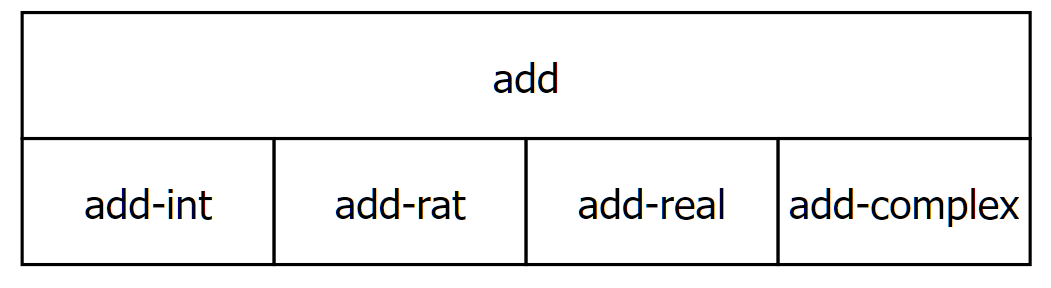
\includegraphics[width=0.8\linewidth]{defaddbeforepoly.png}
  \end{figure}
\end{frame}
% >8-------------------------------TABELA COM PROCEDIMENTOS------------------------------8<


\begin{frame}[fragile]
  \frametitle{Definição do Procedimento \texttt{add}}

  Definição de \texttt{add}:

  \pause
  \vspace{2em}
  Dados de entrada: \texttt{x} \texttt{y}

  \pause
  \vspace{2em}
  \begin{itemize}
    \item Se \texttt{x} e \texttt{y} tiverem o mesmo tipo, então chame o procedimento apropriado na tabela.
  \end{itemize}

\end{frame}


\begin{frame}
  \frametitle{Exemplo de Execução}

\userinput{(add (Z 4) (Z 3))}\\
\useroutput{(Z 7)}

\pause
\vspace{1cm}

\userinput{(add (R 2.4) (R 5.2))}\\
\useroutput{(R 7.6)}

\pause
\vspace{1cm}

\userinput{(add (Q ((Z 3) (Z 2))) (Q ((Z 2) (Z 1))))}\\
\useroutput{(Q ((Z 7) (Z 2)))}

\end{frame}



% >8-----------------------------SOMA ENTRE DIFERENTES TIPOS-----------------------------8<
\begin{frame}[fragile]
  \frametitle{Soma Entre Diferentes Tipos}

  $4 + (5.2 + 2.0i)$ \hfill \texttt{(add (Z 4) (C (R 5.2) (R 2)))}
  \pause
  \vspace{2em}

  \begin{code}
int->complex
  \end{code}

  \pause
  \vspace{2em}

  \begin{code}
int->rat      int->real     int->complex

rat->real     rat->complex

real->complex
  \end{code}

  \pause
  \vspace{2em}
  Próximo a $n^2$ procedimentos em um sistema com $n$ tipos.

\end{frame}
% >8-----------------------------SOMA ENTRE DIFERENTES TIPOS-----------------------------8<



% >8-----------------------------------TORRE DE TIPOS------------------------------------8<
\begin{frame}
  \frametitle{Torre de Tipos}
  \framesubtitle{Hierarquia entre Tipos}
  \only<1>{
    \begin{figure}
      \centering
      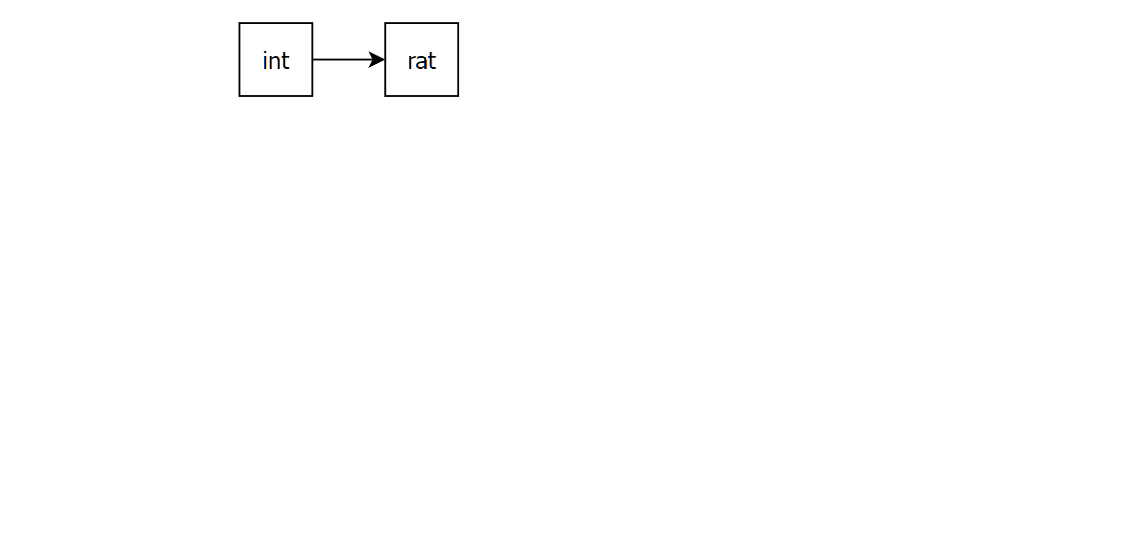
\includegraphics[width=0.8\linewidth]{tower-formation-1.png}
    \end{figure}
    \vspace{1em}
    \vphantom{hey}
  }
  \only<2>{
    \begin{figure}
      \centering
      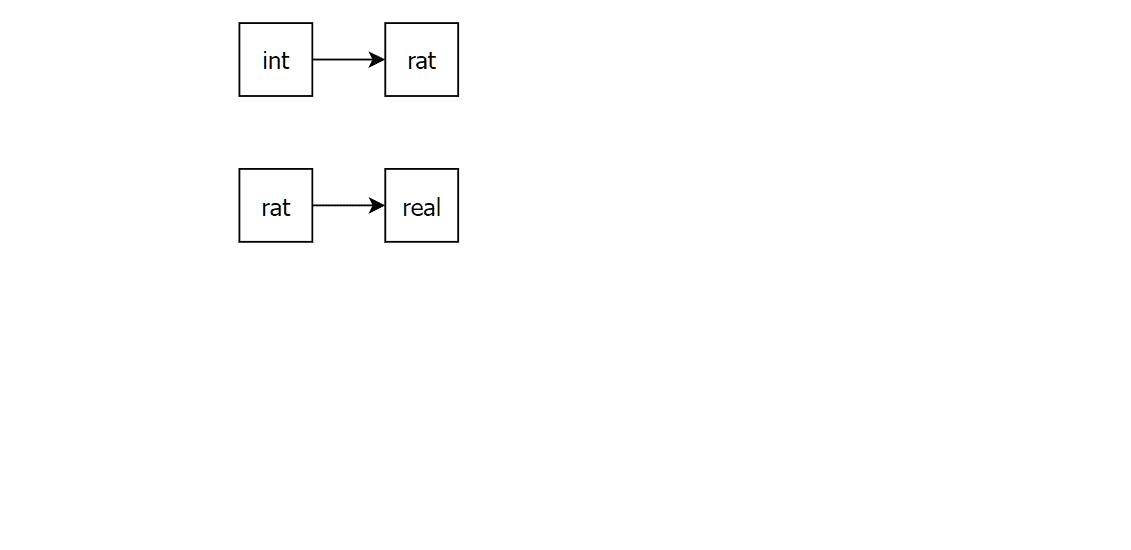
\includegraphics[width=0.8\linewidth]{tower-formation-2.png}
    \end{figure}
    \vspace{1em}
    \vphantom{hey}
  }
  \only<3>{
    \begin{figure}
      \centering
      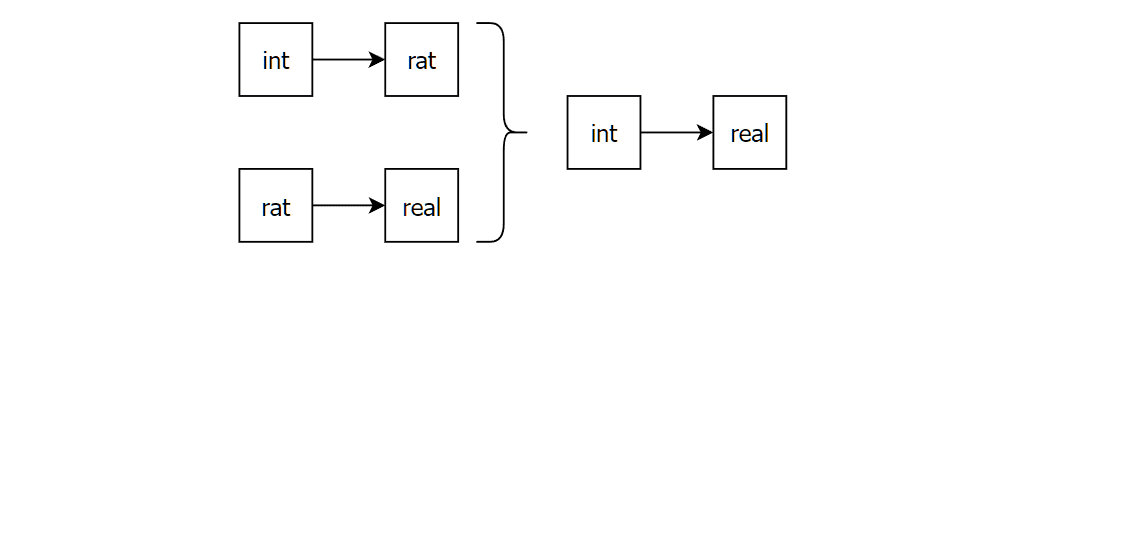
\includegraphics[width=0.8\linewidth]{tower-formation-3.png}
    \end{figure}
    \vspace{1em}
    \vphantom{hey}
  }
  \only<4>{
    \begin{figure}
      \centering
      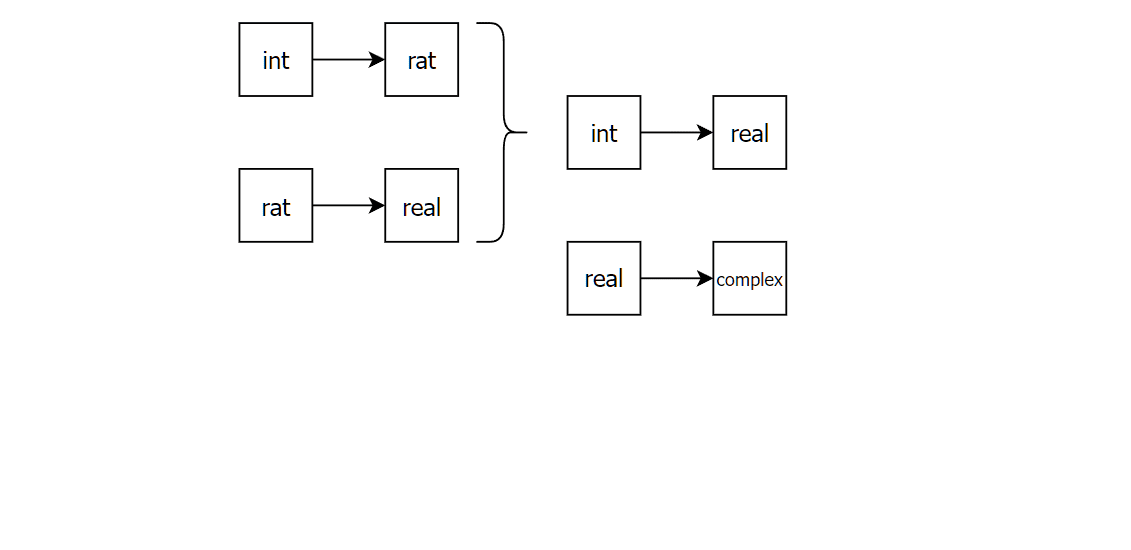
\includegraphics[width=0.8\linewidth]{tower-formation-4.png}
    \end{figure}
    \vspace{1em}
    \vphantom{hey}
  }
  \only<5>{
    \begin{figure}
      \centering
      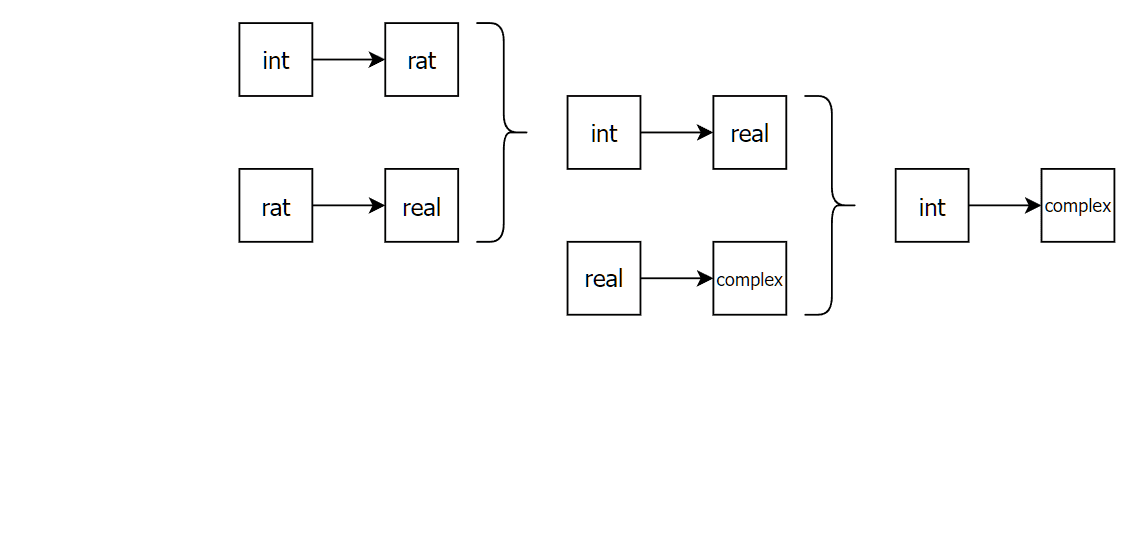
\includegraphics[width=0.8\linewidth]{tower-formation-5.png}
    \end{figure}
    \vspace{1em}
    \vphantom{hey}
  }
  \only<6>{
    \begin{figure}
      \centering
      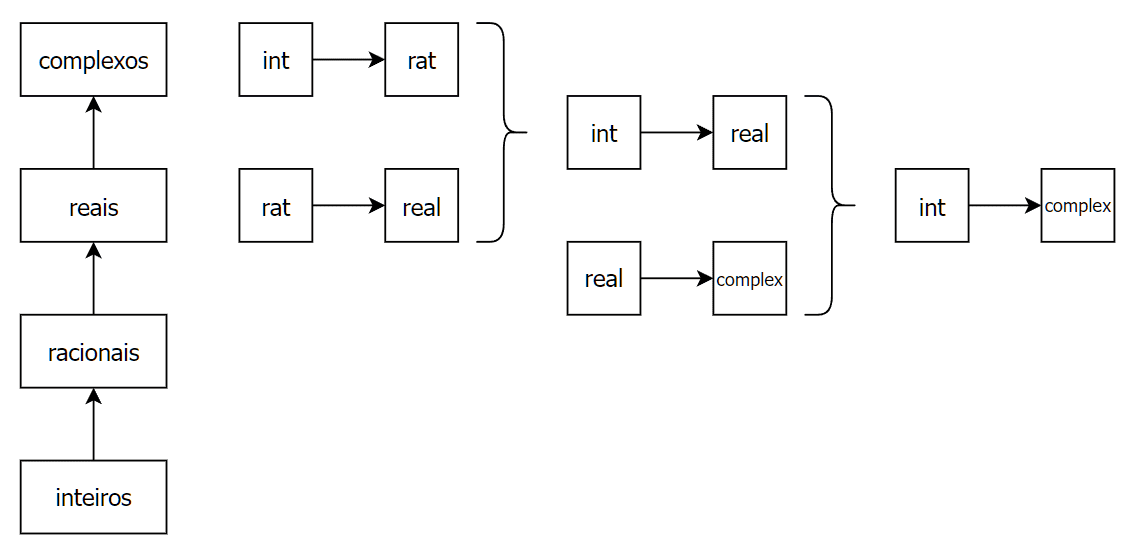
\includegraphics[width=0.8\linewidth]{tower-formation-6.png}
    \end{figure}
    \vspace{1em}
    \vphantom{hey}
  }
  \only<7>{
    \begin{figure}
      \centering
      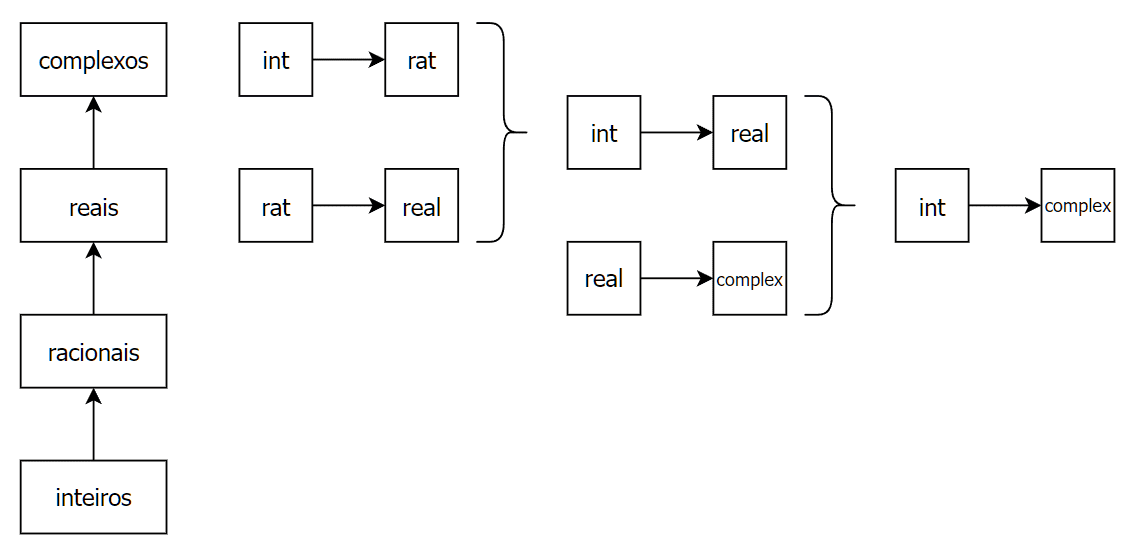
\includegraphics[width=0.8\linewidth]{tower-formation-6.png}
    \end{figure}
    \vspace{1em}
    Próximo a $n$ procedimentos em um sistema com $n$ tipos.
  }
\end{frame}
% >8-----------------------------------TORRE DE TIPOS------------------------------------8<


\begin{frame}[fragile]
  \frametitle{Nova definição do procedimento \texttt{add}}

  Definição de \texttt{add}:

  \pause
  \vspace{2em}
  Dados de entrada: \texttt{x} \texttt{y}

  \pause
  \vspace{2em}
  \begin{itemize}
    \item Se \texttt{x} e \texttt{y} tiverem o mesmo tipo, então chame o procedimento apropriado na tabela;
    \pause
    \item Caso contrário, ``suba a torre'' com o ``menor'' deles e tente somar novamente.
  \end{itemize}

\end{frame}



% >8------------------------EXEMPLO DE EXECUÇÃO DA TORRE DE TIPOS------------------------8<
\begin{frame}
  \frametitle{Exemplo de Execução}
  \framesubtitle{Como a Função add Soma?}
  \only<1>{
    \begin{figure}
      \centering
      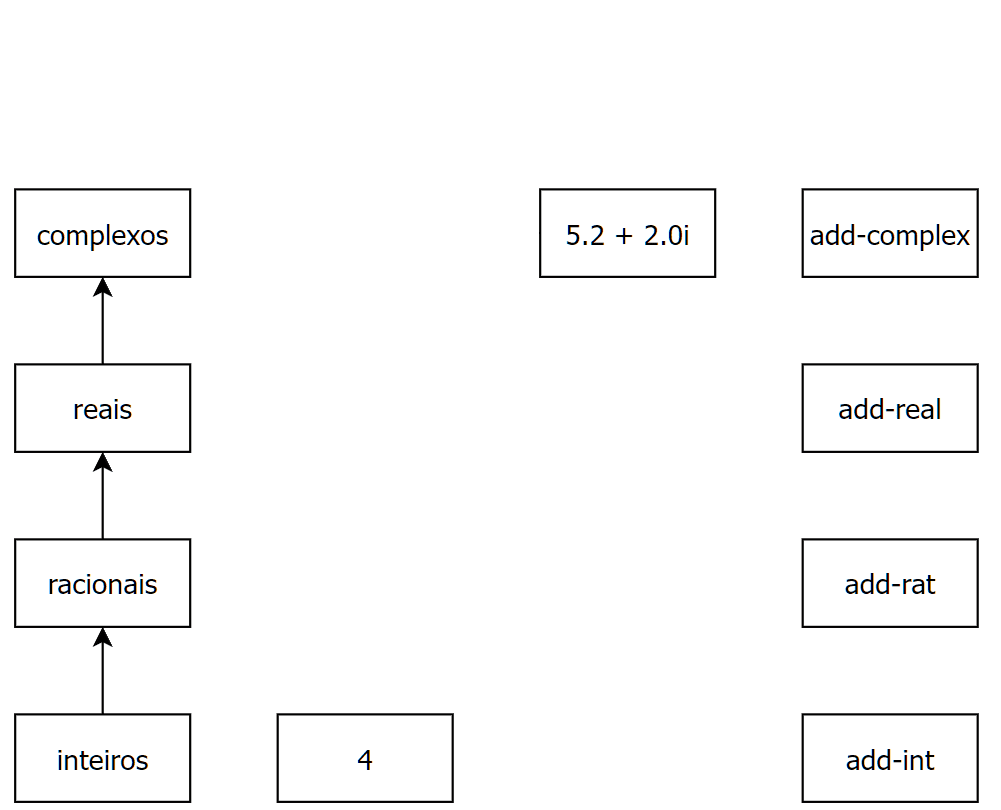
\includegraphics[width=0.7\linewidth]{tower-example-1.png}
    \end{figure}
  }
  \only<2>{
    \begin{figure}
      \centering
      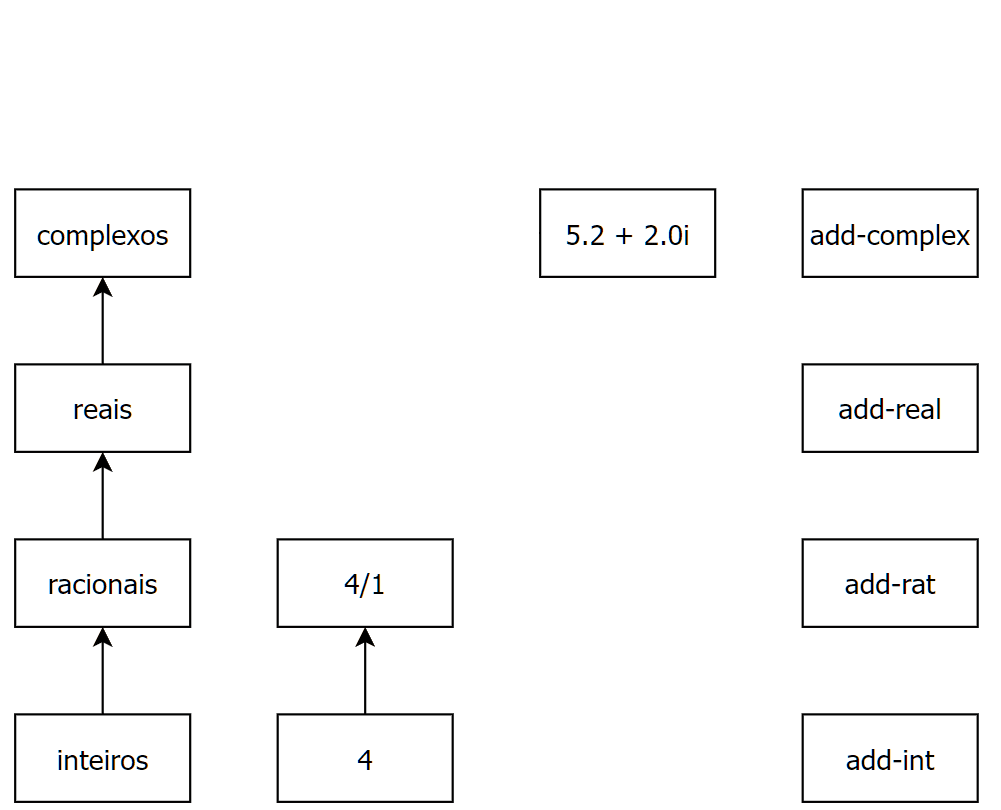
\includegraphics[width=0.7\linewidth]{tower-example-2.png}
    \end{figure}
  }
  \only<3>{
    \begin{figure}
      \centering
      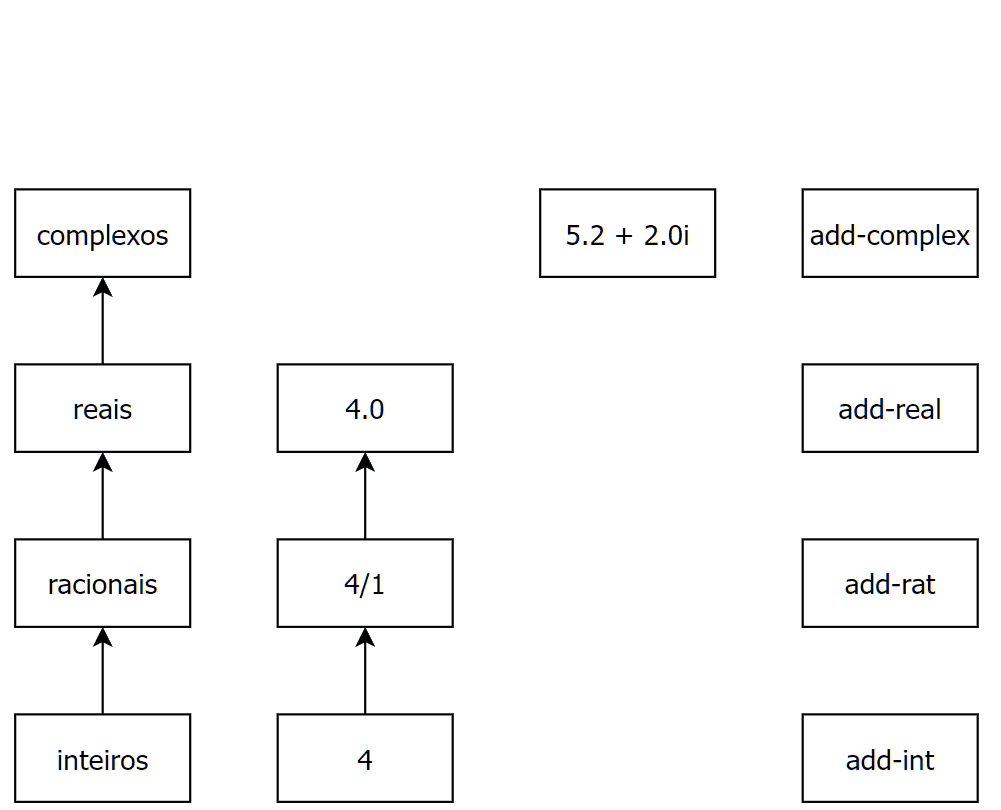
\includegraphics[width=0.7\linewidth]{tower-example-3.png}
    \end{figure}
  }
  \only<4>{
    \begin{figure}
      \centering
      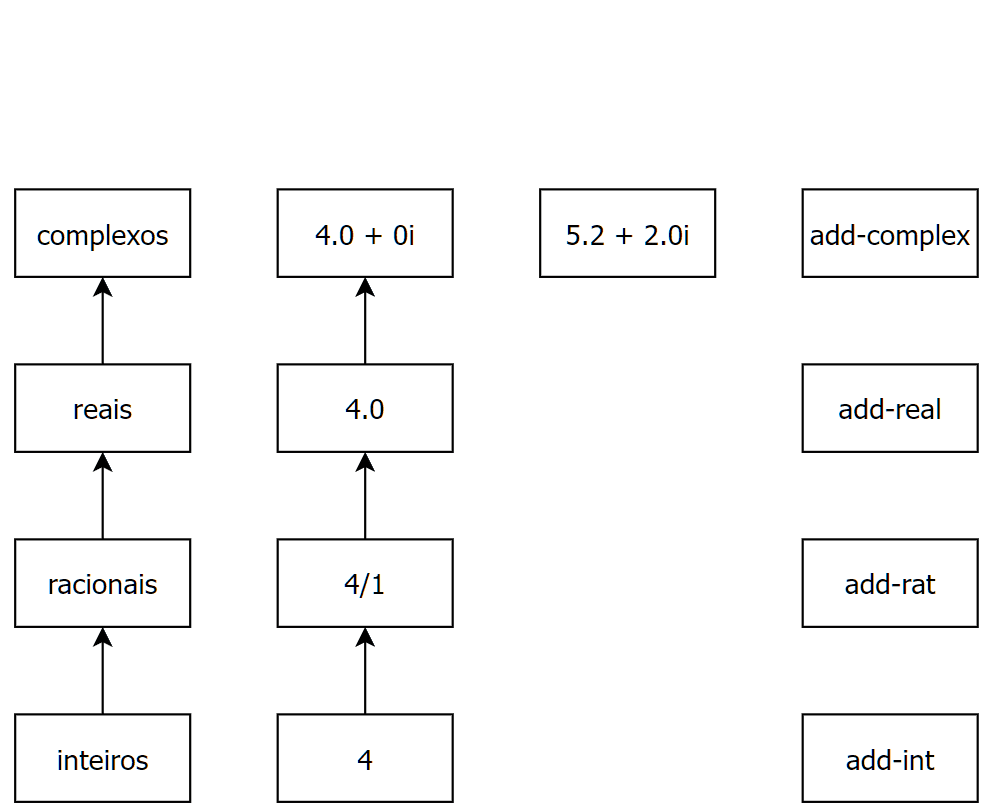
\includegraphics[width=0.7\linewidth]{tower-example-4.png}
    \end{figure}
  }
  \only<5>{
    \begin{figure}
      \centering
      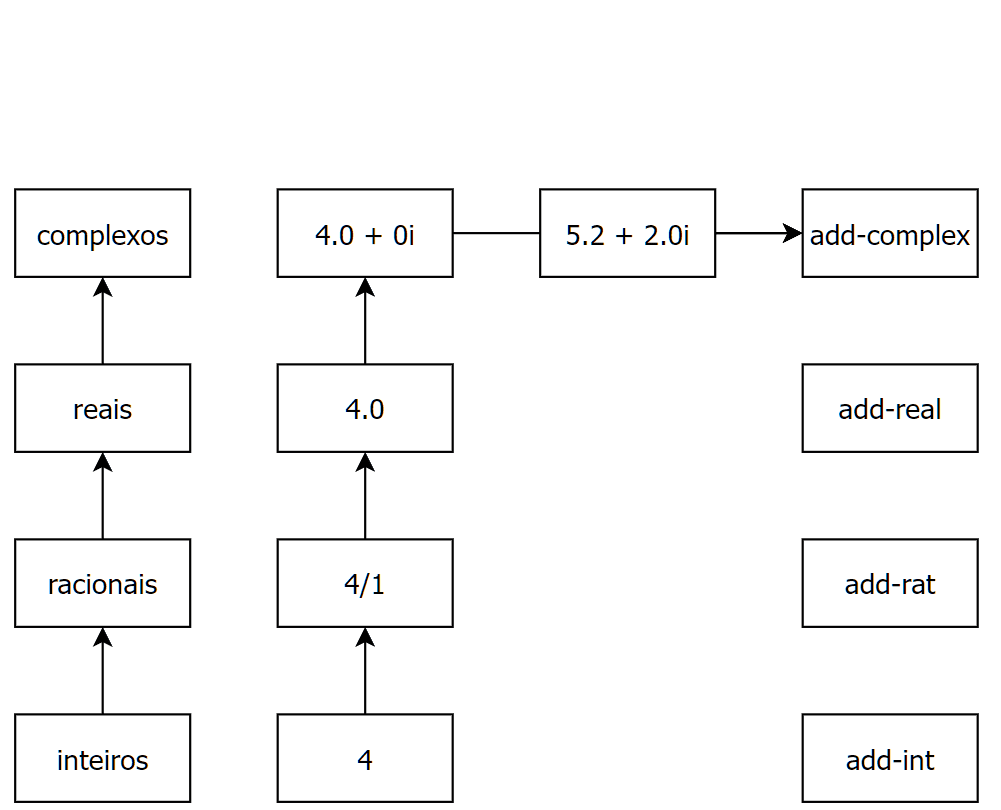
\includegraphics[width=0.7\linewidth]{tower-example-5.png}
    \end{figure}
  }
  \only<6>{
    \begin{figure}
      \centering
      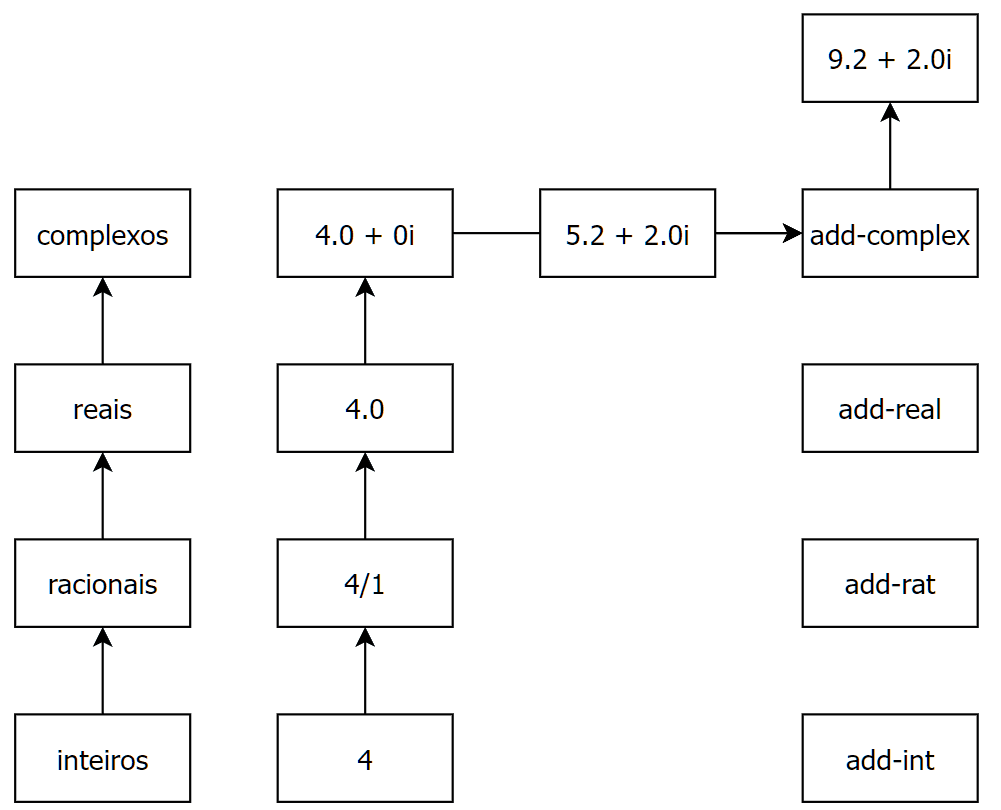
\includegraphics[width=0.7\linewidth]{tower-example-6.png}
    \end{figure}
  }
\end{frame}
\begin{frame}
  \begin{figure}
    \centering
    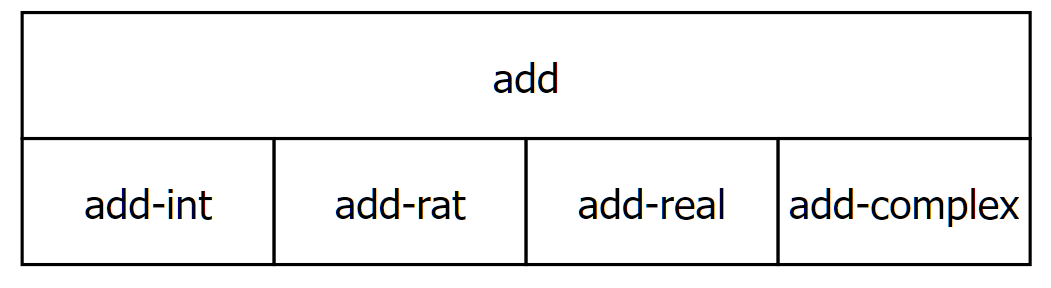
\includegraphics[width=0.8\linewidth]{defaddbeforepoly.png}
  \end{figure}
\end{frame}
% >8------------------------EXEMPLO DE EXECUÇÃO DA TORRE DE TIPOS------------------------8<



% >8-----------------------------EXTENSIBILIDADE (POLINÔMIOS)----------------------------8<
\section{Extensibilidade}
\begin{frame}
  \frametitle{Polinômios}
  \begin{center}
    E se quisermos estender nosso \\
    sistema para que inclua polinômios?
  \end{center}
\end{frame}



\begin{frame}
  \frametitle{Soma de Polinômios}

  $(4x^0 + 2x^2) + (2x^0 + 1x^1 + 5x^2)$\\
  \pause
  \vspace{2em}
  $= (4 + 2)x^0 + 1x^1 + (2 + 5)x^2$\\
  \pause
  \vspace{2em}
  $= 6x^0 + 1x^1 + 7x^2$
\end{frame}



\begin{frame}[fragile]
  \begin{code}
(define (add-poly p1 p2)
  <...>
  (if (= (exp p1) (exp p2))
      (+ (coeff p1) (coeff p2))
      <...>))
  \end{code}
\end{frame}



\begin{frame}[fragile]
  \begin{code}
(define (add-poly p1 p2)
  <...>
  (if (= (exp p1) (exp p2))
      (add (coeff p1) (coeff p2))
      <...>))
  \end{code}
\end{frame}



\begin{frame}[fragile]
  \[2x^1 + \left(\dfrac{4}{3}\right)x^2 + 5.2x^4 + (3.4 + 2.5i)x^5\]

  \pause
  \vspace{2em}
  \begin{center}
    Mas e se inserirmos \texttt{add-poly} na tabela?
  \end{center}
\end{frame}


\begin{frame}
  \frametitle{Nova Definição de \texttt{add}}
  \begin{figure}
    \centering
    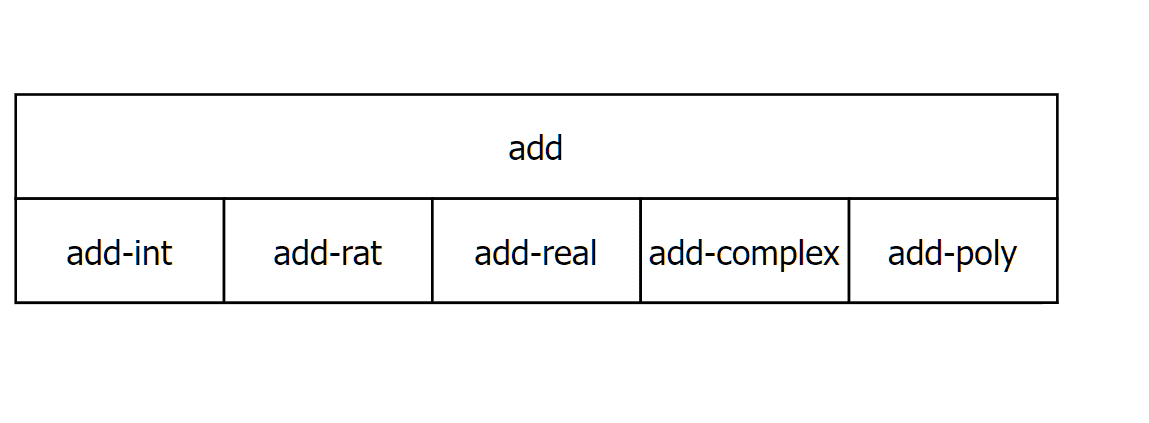
\includegraphics[width=1\linewidth]{defaddinit.png}
  \end{figure}
\end{frame}


\begin{frame}[fragile]
  \frametitle{Recaptulando Definições}
  \begin{code}
(define (add-int x y)
  (cons Z (+ (cdr x)
             (cdr y))))
  \end{code}
  \pause
  \vspace{1em}

  \begin{code}
(define (add-poly p1 p2)
  <...>
  (if (= (exp p1) (exp p2))
      (add (coeff p1) (coeff p2))
      <...>))
  \end{code}
\end{frame}



\begin{frame}
  \frametitle{Nova Definição de add}
  \only<1>{
    \begin{figure}
      \centering
      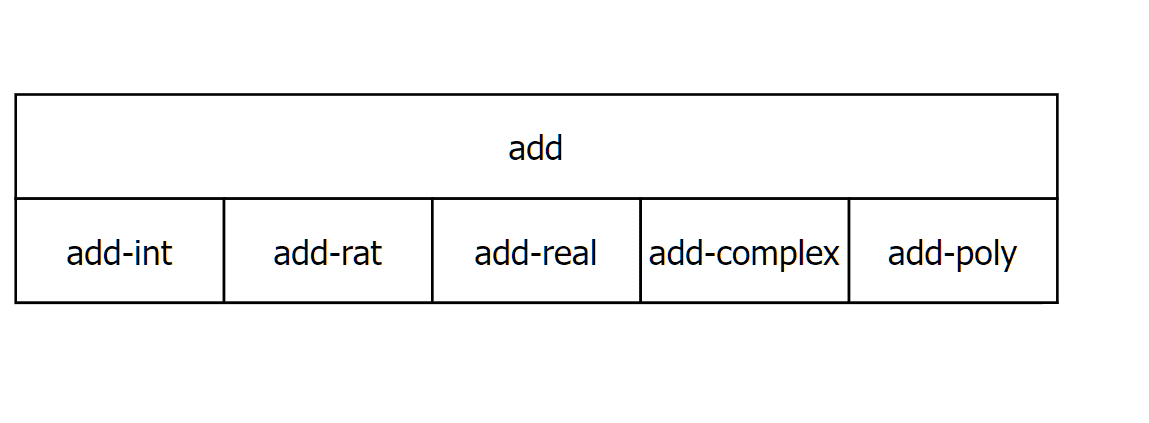
\includegraphics[width=1\linewidth]{defaddinit.png}
    \end{figure}
  }
  \only<2>{
    \begin{figure}
      \centering
      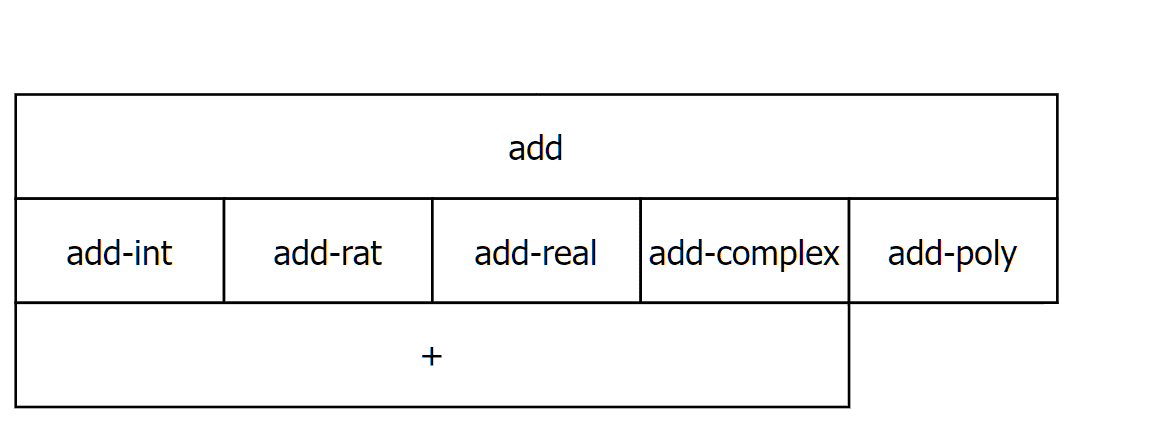
\includegraphics[width=1\linewidth]{defaddmid.png}
    \end{figure}
  }
  \only<3>{
    \begin{figure}
      \centering
      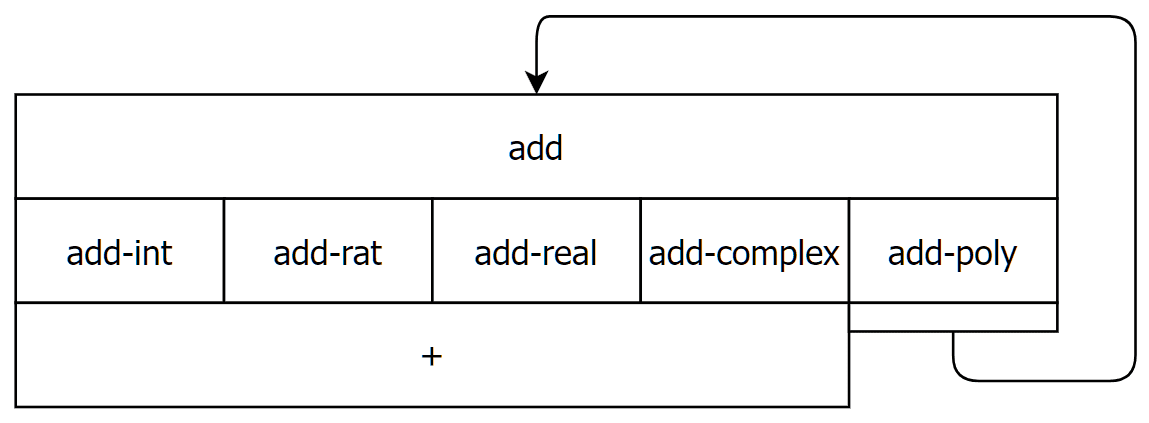
\includegraphics[width=1\linewidth]{defaddfinal.png}
    \end{figure}
  }
\end{frame}



\begin{frame}
  \frametitle{Polinômios de Polinômios}

  Agora podemos construir polinômios que tenham formatos como:

  \vspace{2em}

  \[(\left(\dfrac{1}{2}\right)x^1 + (2z^1 + 3z^5)x^3 + 8x^4)y^2 + (4x^0 + 10.5x^1)y^3\]
\end{frame}


\begin{frame}
  \frametitle{Matrizes}
  \begin{center}
    E se quisermos estender nosso \\
    sistema para que inclua matrizes?
  \end{center}
\end{frame}

\begin{frame}
  \frametitle{Soma de Matrizes}

  \only<1>{
  \[\begin{bmatrix}
    a & b \\ c & d
  \end{bmatrix} +
  \begin{bmatrix}
    x & y \\ z & w
  \end{bmatrix} =
  \begin{bmatrix}
    a+x & b+y \\ c+z & d+w
  \end{bmatrix}\]
  }
  \only<2>{
    \[\begin{bmatrix}
    a & b \\ c & d
  \end{bmatrix}
  \texttt{ add }
  \begin{bmatrix}
    x & y \\ z & w
  \end{bmatrix} =
  \begin{bmatrix}
    a \texttt{ add } x & b \texttt{ add } y \\ c \texttt{ add } z & d \texttt{ add } w
  \end{bmatrix}\]
  }
\end{frame}

\begin{frame}[fragile]
  \[\begin{pmatrix}
    2x^0 + (5.4y^2)x^2 &  & 5y^1 + \left(\dfrac{3}{4}x^2\right)y^3 \\
    \\
    8.9z^3 + (1.3w^7)z^5 &  &(4.3 + 2.1i)h^2 + 5h^3
  \end{pmatrix}\]
\end{frame}

\begin{frame}
  \begin{figure}
    \centering
    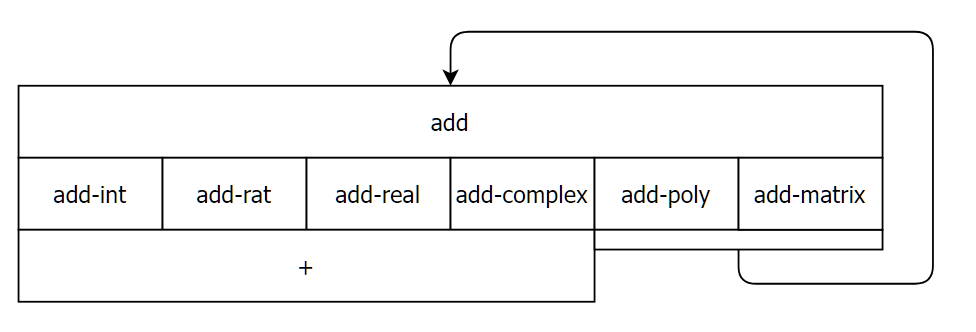
\includegraphics[width=\linewidth]{defaddmatrix.png}
  \end{figure}
\end{frame}


% >8-----------------------------EXTENSIBILIDADE (POLINÔMIOS)----------------------------8<
